\documentclass[11pt]{beamer}
\usetheme{Warsaw}
\usepackage[utf8]{inputenc}
\usepackage[english]{babel}
\usepackage{tikz}
\usetikzlibrary{shapes,arrows}
\usepackage{amsmath,bm,times}
\usetikzlibrary{shapes,snakes,arrows,shadows}
\usetikzlibrary{matrix}
\usetikzlibrary{shapes.geometric}
\usetikzlibrary{positioning}
\usepackage{subcaption}

\setbeamercovered{transparent} 
%animation
\tikzset{
  invisible/.style={opacity=0.2},
  visible on/.style={alt={#1{}{invisible}}},
  alt/.code args={<#1>#2#3}{%
    \alt<#1>{\pgfkeysalso{#2}}{\pgfkeysalso{#3}} % \pgfkeysalso doesn't change the path
  },
}


%
\newcommand{\mx}[1]{\mathbf{\bm{#1}}} % Matrix command
\newcommand{\vc}[1]{\mathbf{\bm{#1}}} % Vector command

% We need layers to draw the block diagram
\pgfdeclarelayer{background}
\pgfdeclarelayer{foreground}
\pgfsetlayers{background,main,foreground}

% Define a few styles and constants
\tikzstyle{sensor}=[draw, fill=blue!20,rounded corners, text width=5em, 
    text centered, minimum height=2.5em]
\tikzstyle{block}=[sensor,visible on=<#1->]

\tikzstyle{input}=[fill=blue!20, regular polygon, regular polygon sides=3,rotate=-90,visible on=<#1->]
\tikzstyle{ann} = [above, text width=5em,visible on=<#1->]
\tikzstyle{naveqs} = [sensor, text width=6em, fill=black!20, 
    minimum height=12em, rounded corners,visible on=<#1->]
\tikzstyle{psola} = [sensor, text width=4em, fill=green!40, 
    minimum height=10em, rounded corners,visible on=<#1->]


\def\blockdist{4.3}
\def\edgedist{1.2}




\begin{document}
%% Slide 1
\begin{frame}
\begin{figure}
\begin{subfigure}{.5\textwidth}
  \centering
  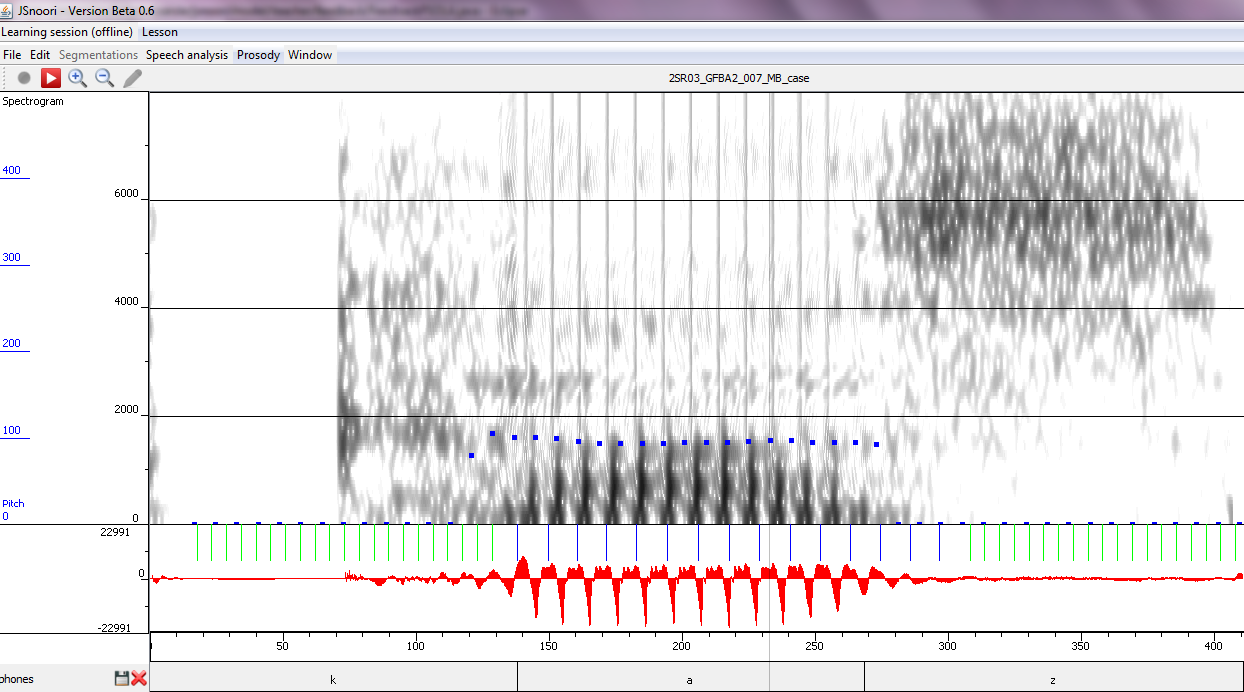
\includegraphics[width=0.9\linewidth]{images/case_learner.PNG}
  \caption{Learner signal before feedback correction}
  \label{fig:sfig1}
\end{subfigure}%
\begin{subfigure}{.5\textwidth}
  \centering
  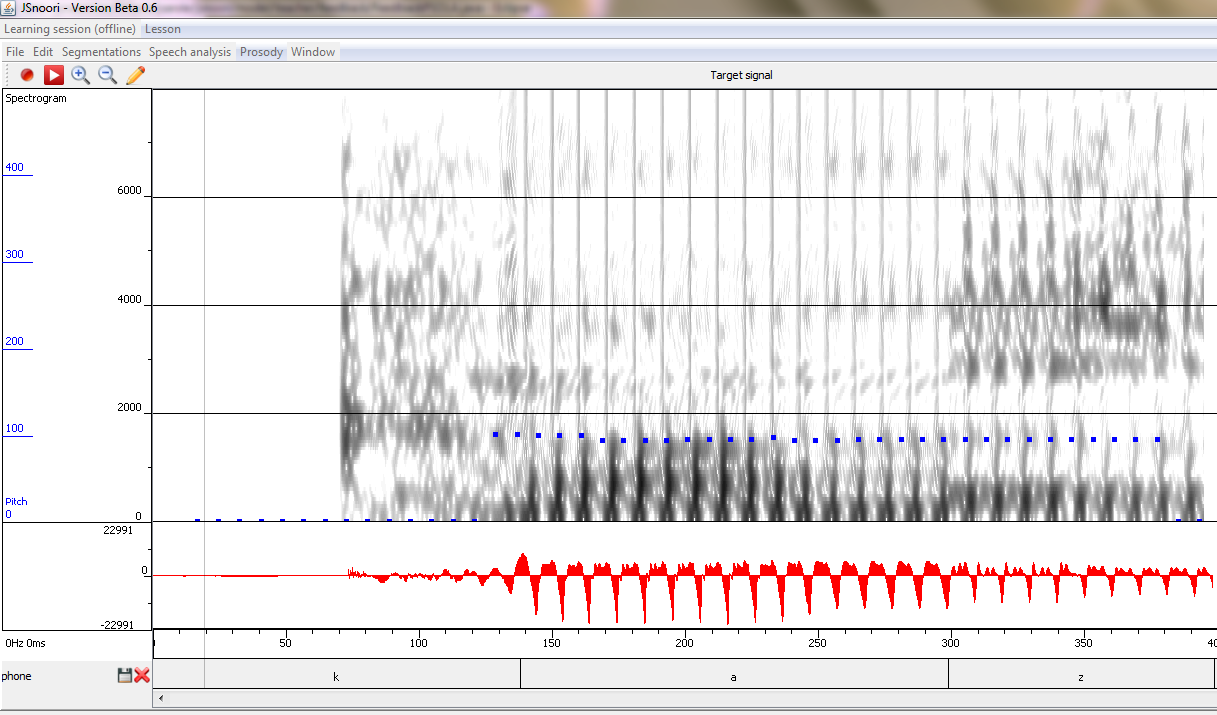
\includegraphics[width=0.86\linewidth]{images/case_target_2.PNG}
  \caption{Learner signal after feedback correction}
  \label{fig:sfig2}
\end{subfigure}
\caption{Feedback Correction : example Word \emph{case}}
\label{fig:fig}
\end{figure}
\end{frame}


% Slide 2
\begin{frame}

\begin{figure}
\begin{subfigure}{.5\textwidth}
  \centering
  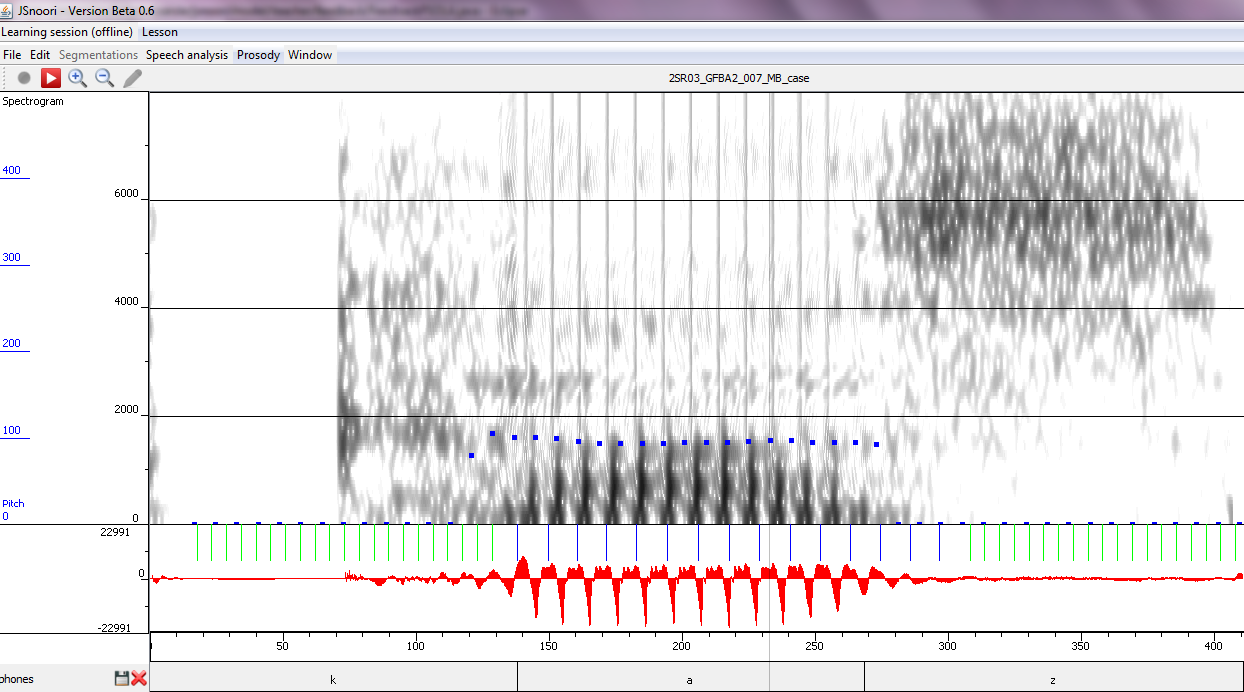
\includegraphics[width=0.9\linewidth]{images/case_learner.PNG}
  \caption{Learner signal before feedback correction}
  \label{fig:sfig1}
\end{subfigure}%
\begin{subfigure}{.5\textwidth}
  \centering
  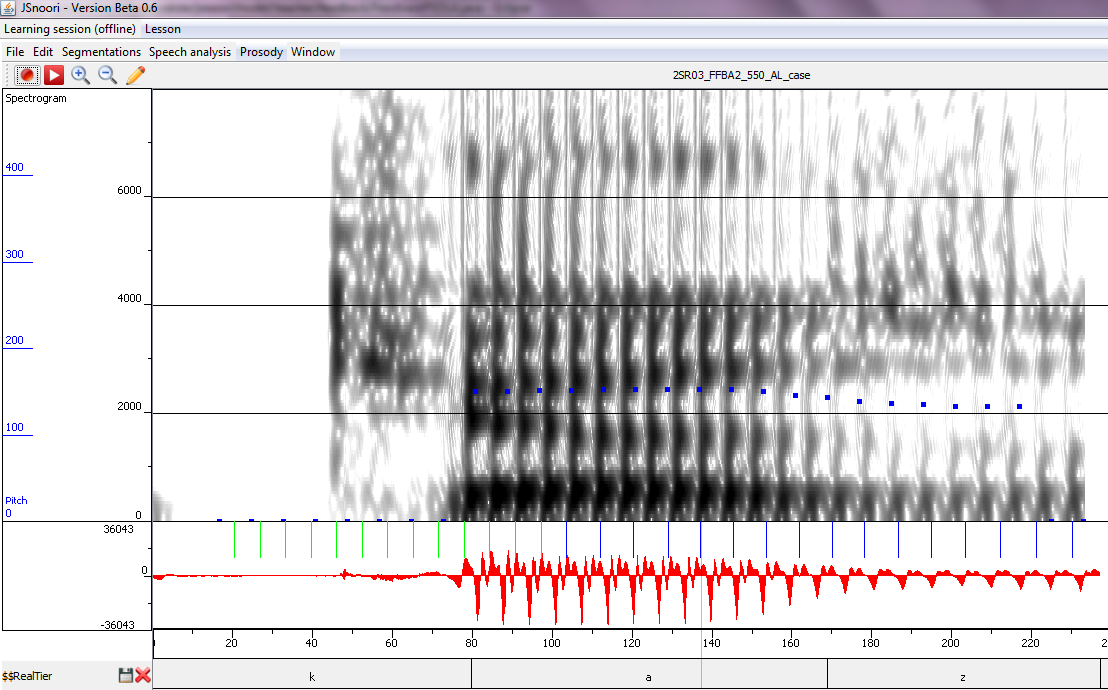
\includegraphics[width=0.87\linewidth]{images/teacher_case.PNG}
  \caption{Teacher Signal}
  \label{fig:sfig2}
\end{subfigure}
\caption{Feedback Correction : example Word \emph{case}}
\label{fig:fig}
\end{figure}
\end{frame}

%%% Slide 3
\begin{frame}

\begin{figure}
\begin{subfigure}{.5\textwidth}
  \centering
  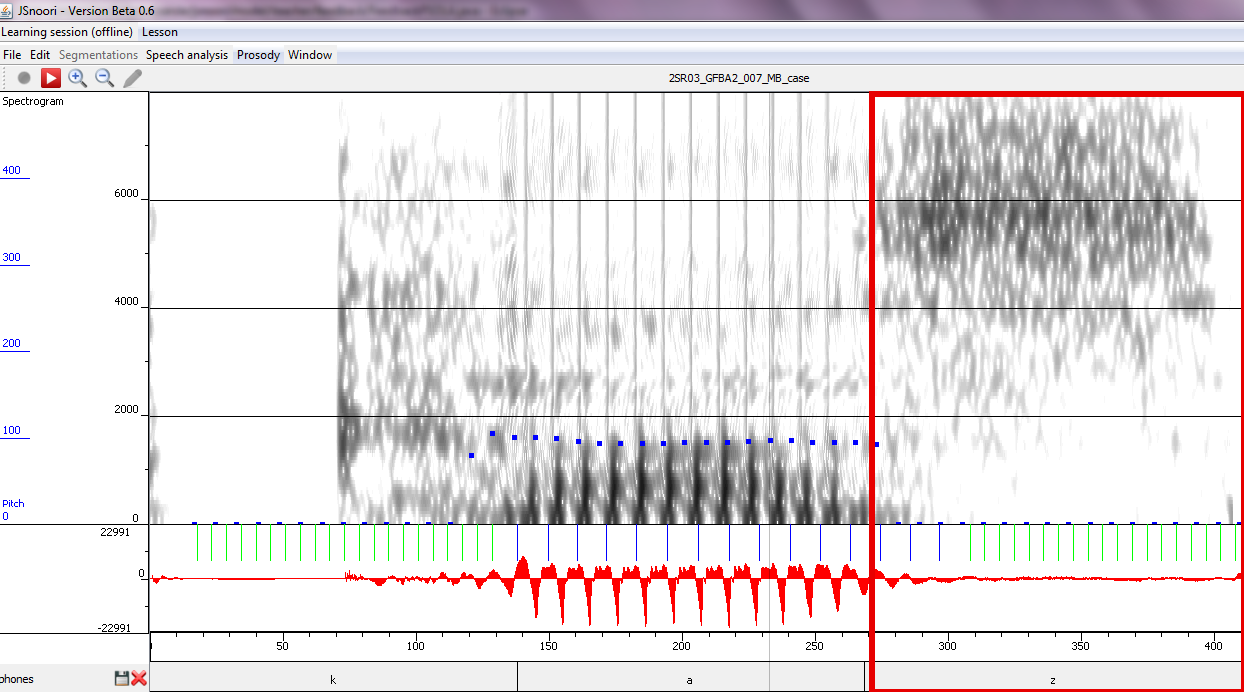
\includegraphics[width=0.9\linewidth]{images/case_learner-changed.PNG}
  \caption{Learner signal before feedback correction}
  \label{fig:sfig1}
\end{subfigure}%
\begin{subfigure}{.5\textwidth}
  \centering
  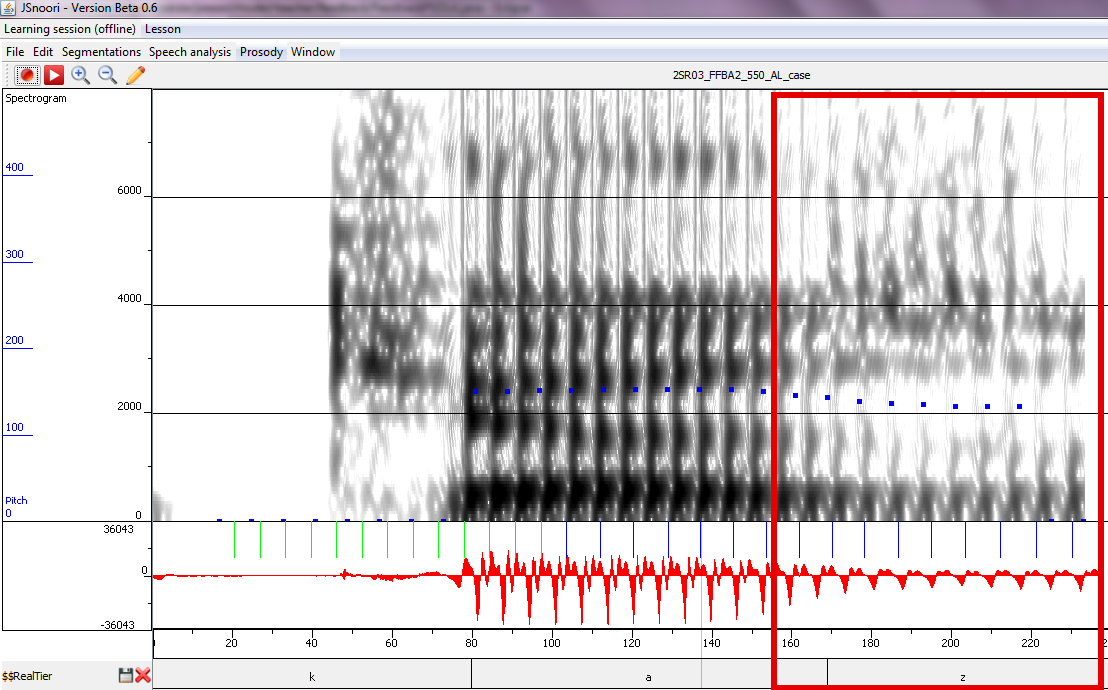
\includegraphics[width=0.9\linewidth]{images/teacher_case_Changed.PNG}
  \caption{Teacher signal}
  \label{fig:sfig2}
\end{subfigure}
\caption{Feedback Correction : example Word \emph{case}}
\label{fig:fig}
\end{figure}
\end{frame}


%Slide 4
\begin{frame}

\begin{figure}
\begin{subfigure}{.5\textwidth}
  \centering
  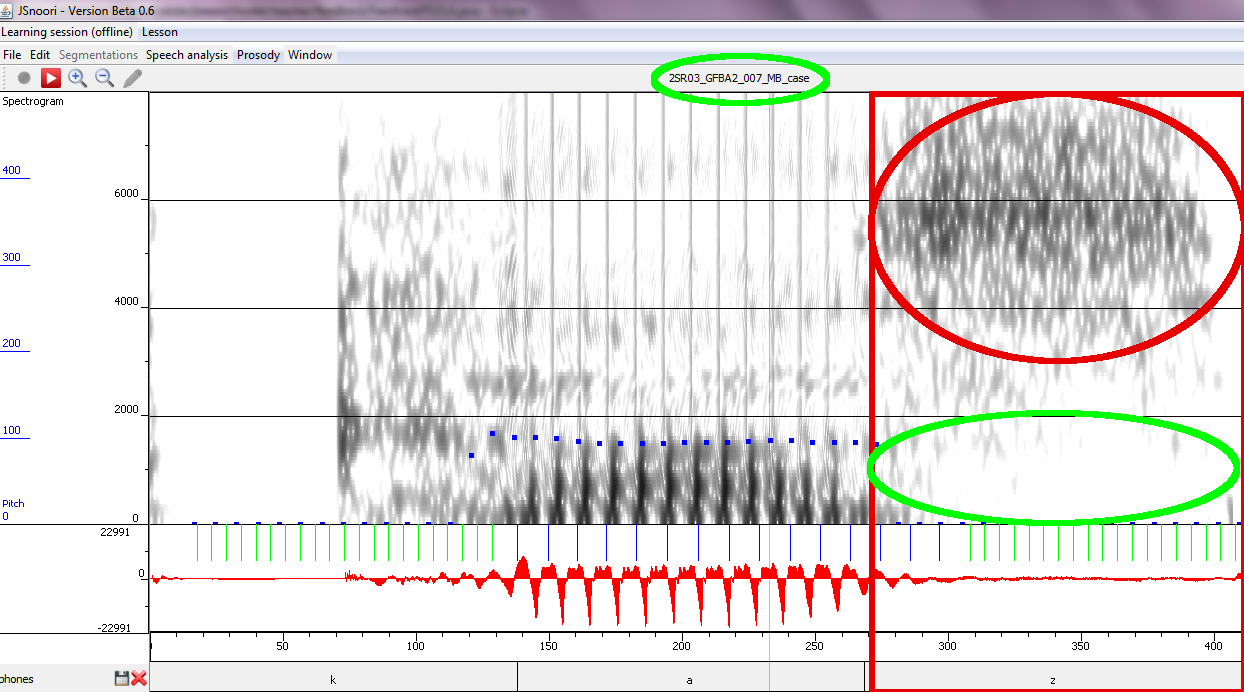
\includegraphics[width=0.9\linewidth]{images/case_learner-changed2.PNG}
  \caption{Learner signal before feedback correction}
  \label{fig:sfig1}
\end{subfigure}%
\begin{subfigure}{.5\textwidth}
  \centering
  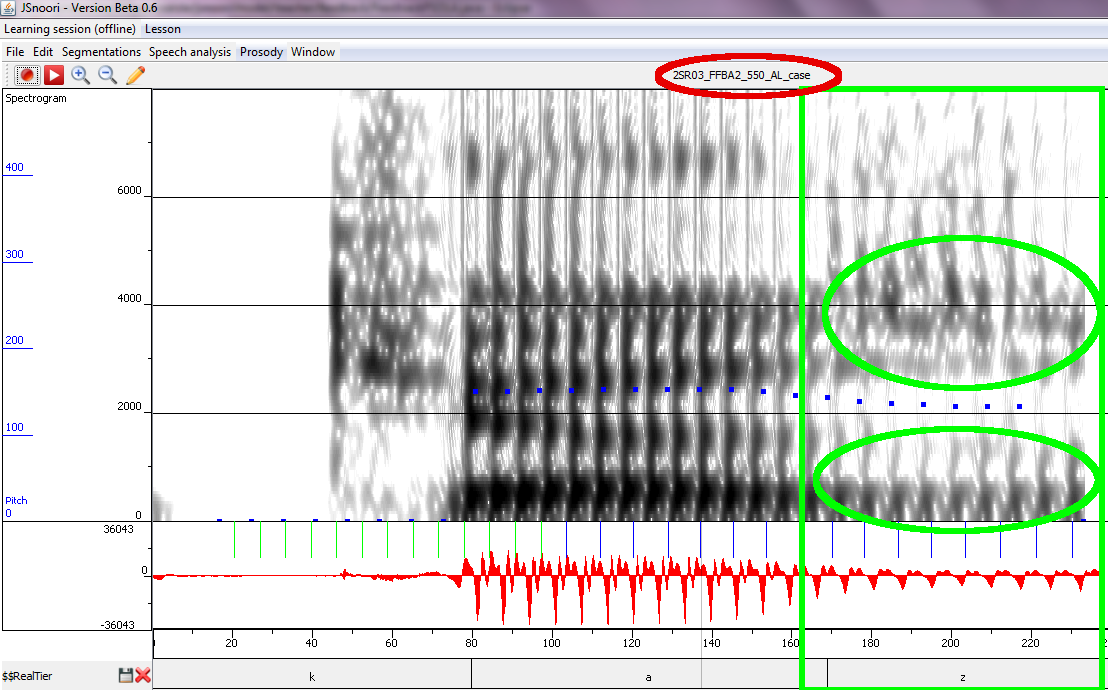
\includegraphics[width=0.9\linewidth]{images/teacher_case_changed2.PNG}
  \caption{Teacher signal}
  \label{fig:sfig2}
\end{subfigure}
\caption{Feedback Correction : example Word \emph{case}}
\label{fig:fig}
\end{figure}
\end{frame}

%% Slide 5
\begin{frame}
\begin{figure}

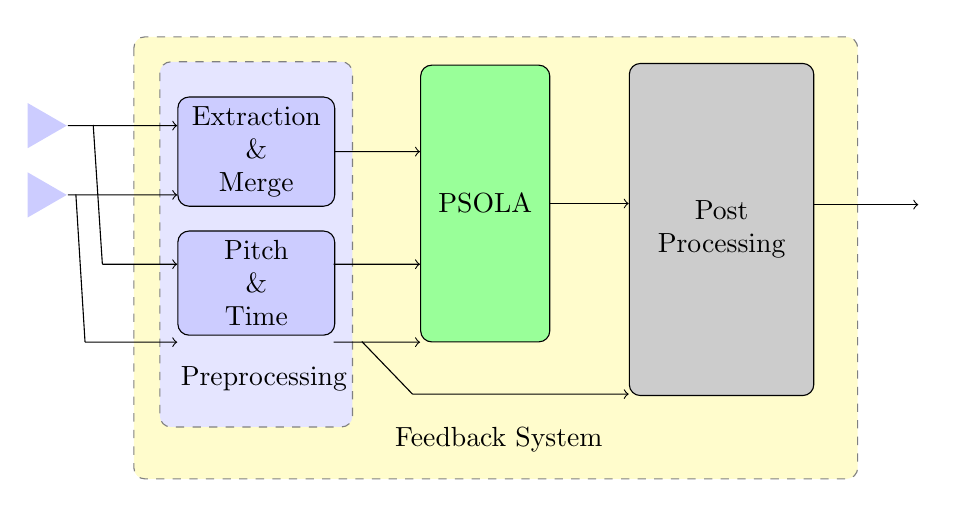
\begin{tikzpicture}[scale=1.1]
    \node (naveq) [naveqs={1}] {Post \\ Processing};
    % Note the use of \path instead of \node at ... below. 
     	
 	\path (naveq.0)+(-3.8,+0.3) node (psola) [psola={1}] {PSOLA};
      
    \path (naveq.140)+(-\blockdist,0) node (gyros) [block={1}] {Extraction \\ \& \\ Merge};
    \path (naveq.-150)+(-\blockdist,0) node (accel) [block={1}] {Pitch \\ \& \\ Time };
	\path (gyros.0)+(-3.4,+0.3) node (teacher) [input={1}] {};
    \path (gyros.0)+(-3.4,-0.5) node (learner) [input={1}] {};
 	
\path [draw, ->] (teacher) -- node [above] {} 
        (gyros.west |- teacher);
\path [draw, ->] (learner) -- node [above] {} 
        (gyros.west |- learner);
%\draw[<-] (accel.west) -- +(-0.8,0);
%\draw[<-] (accel.west) -- +(-0.8,0	);
\path (gyros.0)+(-2.8,-1.30) node (ref1){}; 
\path (gyros.0)+(-3.0,-2.2) node (ref2){};
%
\path (gyros.0)+(-2.8,+0.42) node (refTeacher){}; 
\path (gyros.0)+(-3.0,-0.38) node (refLearner){};
%
\path (gyros.east)+(-0.13,-1.30) node (pitch){}; 
\path (gyros.east)+(-0.13,-2.2) node (time){};
%
\path (gyros.east)+(+0.2,-2.080) node (ref1Pitch){}; 
\path (psola.west)+(-0.2,-2.2) node (ref2Pitch){}; 

%
%
%    \draw[->] (branch) node[branch] {}{}|- (ref1)




\path [draw, ->] (ref1) -- node [above] {} 
        (accel.west |- ref1);
 
\path [draw, ->] (ref2) -- node [above] {} 
        (accel.west |- ref2);

\path [draw, ->] (gyros) -- node [above] {} 
        (psola.west |- gyros);

\path [draw, -] (refTeacher)--(ref1.east);

\path [draw, -] (refLearner) -- (ref2.east);

\path [draw, ->] (pitch) -- node [above] {} 
        (psola.west |- pitch);

\path [draw, ->] (time) -- node [above] {} 
        (psola.west |- time);

\path [draw, ->] (ref2Pitch) -- node [above] {} 
        (naveq.west |- ref2Pitch);

\path [draw, -] (ref1Pitch) -- (ref2Pitch.east);

\path [draw, ->] (psola.east) -- node [above] {} 
        (naveq.west |- psola.east);
  
    % Unfortunately we cant use the convenient \path (fromnode) -- (tonode) 
    % syntax here. This is because TikZ draws the path from the node centers
    % and clip the path at the node boundaries. We want horizontal lines, but
    % the sensor and naveq blocks aren't aligned horizontally. Instead we use
    % the line intersection syntax |- to calculate the correct coordinate
   % \path [draw, ->] (gyros) -- node [above] {$\vc{\omega}_{ib}^b$} 
    %    (naveq.west |- gyros) ;
    % We could simply have written (gyros) .. (naveq.140). However, it's
    % best to avoid hard coding coordinates
    \path (accel.south west)+(+1.0,-0.5) node (IMU) {Preprocessing};
    \path (naveq.south west)+(-1.5,-0.5) node (INS) {Feedback System};
    \draw [->] (naveq.15	) -- node [ann={1}] {} + (\edgedist,0) 
        node[right] {};
%    \draw [->] (naveq.20) -- node [ann] {Attitude} + (\edgedist,0) 
   %     node[right] { $\mx{R}_l^b$};
%    \draw [->] (naveq.-25) -- node [ann] {Horisontal position} + (\edgedist,0)
   %     node [right] {$\mx{R}_e^l$};
%    \draw [->] (naveq.-50) -- node [ann] {Depth} + (\edgedist,0) 
%        node[right] {$z$};
    
    % Now it's time to draw the colored IMU and INS rectangles.
    % To draw them behind the blocks we use pgf layers. This way we  
    % can use the above block coordinates to place the backgrounds   
    \begin{pgfonlayer}{background}
        % Compute a few helper coordinates
        \path (gyros.west |- naveq.north)+(-0.5,0.3) node (a) {};
        \path (INS.south -| naveq.east)+(+0.5,-0.2) node (b) {};
        \path[fill=yellow!20,rounded corners, draw=black!50, dashed]
            (a) rectangle (b);
        \path (gyros.north west)+(-0.2,0.4) node (a) {};
        \path (IMU.south -| gyros.east)+(+0.2,-0.3) node (b) {};
        \path[fill=blue!10,rounded corners, draw=black!50, dashed]
            (a) rectangle (b);
    \end{pgfonlayer}
\end{tikzpicture}
\caption{Schema Block of Feedback Correction System }
\end{figure}
	\end{frame}
	
%% slide extraction pitch mark;

\begin{frame}

\begin{figure}
\begin{subfigure}{.5\textwidth}
  \centering
  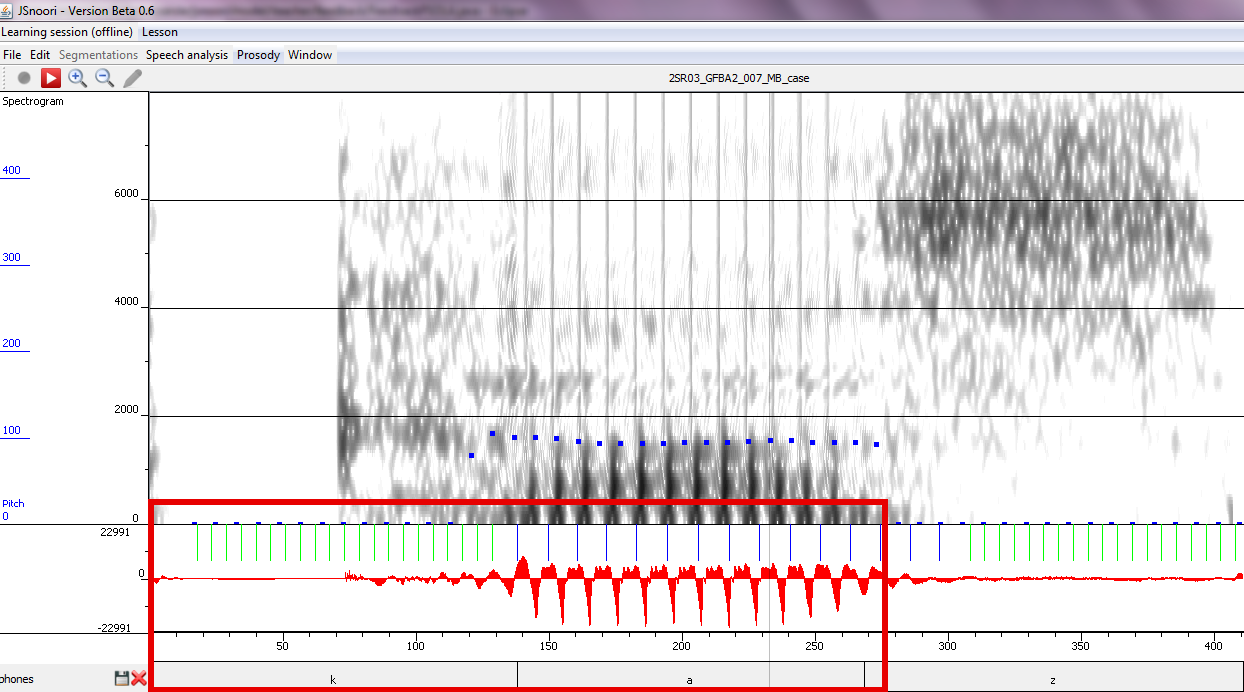
\includegraphics[width=0.9\linewidth]{images/case_learner-nonFricative.PNG}
  \caption{Pitch markers no-fricative extraction from the learner}
  \label{fig:sfig1}
\end{subfigure}%
\begin{subfigure}{.5\textwidth}
  \centering
  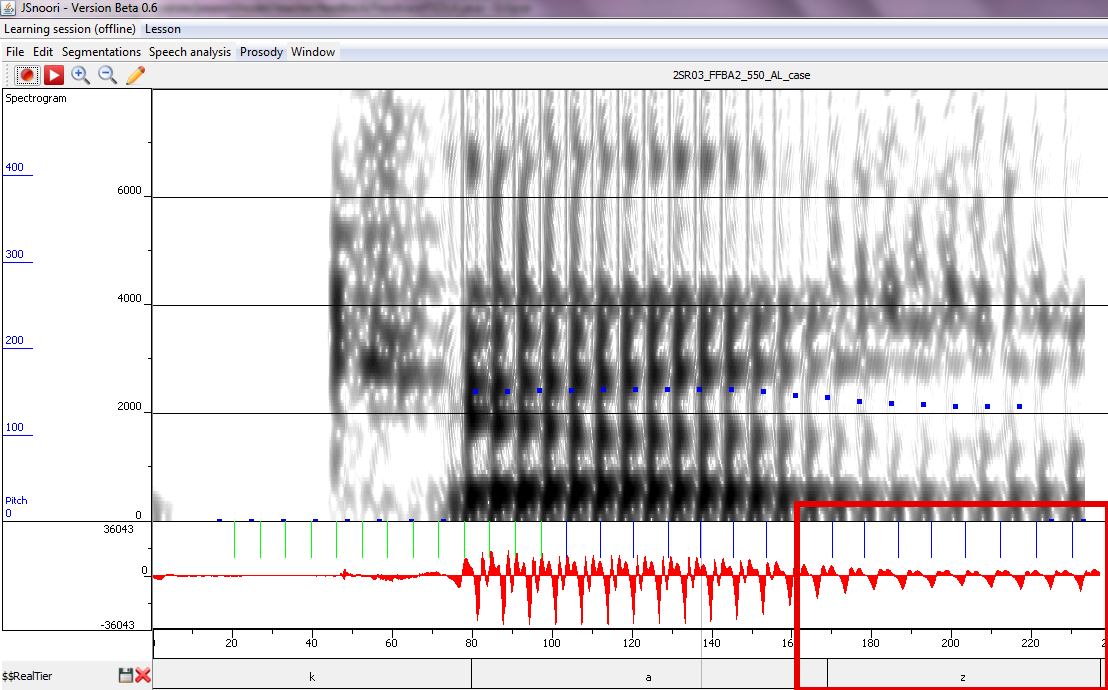
\includegraphics[width=0.9\linewidth]{images/teacher_case_pitchMarks.PNG}
  \caption{Pitch markers fricative extraction from the teacher}
  \label{fig:sfig2}
\end{subfigure}
\caption{Pitch Mark Extraction}
\label{fig:fig}
\end{figure}
\end{frame}
%% slide pitch & time 
\begin{frame}
%
\begin{figure}
%%%%%
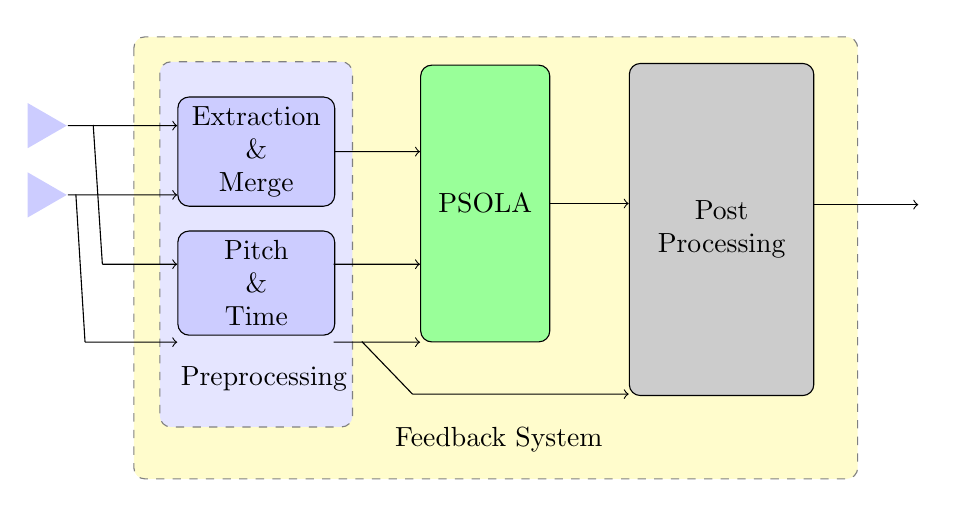
\begin{tikzpicture}[scale=1.1]
    \node (naveq) [naveqs={2}] {Post \\ Processing};
    % Note the use of \path instead of \node at ... below. 
     	
 	\path (naveq.0)+(-3.8,+0.3) node (psola) [psola={2}] {PSOLA};
      
    \path (naveq.140)+(-\blockdist,0) node (gyros) [block={1}] {Extraction \\ \& \\ Merge};
    \path (naveq.-150)+(-\blockdist,0) node (accel) [block={2}] {Pitch \\ \& \\ Time };
	\path (gyros.0)+(-3.4,+0.3) node (teacher) [input={1}] {};
    \path (gyros.0)+(-3.4,-0.5) node (learner) [input={1}] {};
 	
\path [draw, ->] (teacher) -- node [above] {} 
        (gyros.west |- teacher);
\path [draw, ->] (learner) -- node [above] {} 
        (gyros.west |- learner);
%\draw[<-] (accel.west) -- +(-0.8,0);
%\draw[<-] (accel.west) -- +(-0.8,0	);
\path (gyros.0)+(-2.8,-1.30) node (ref1){}; 
\path (gyros.0)+(-3.0,-2.2) node (ref2){};
%
\path (gyros.0)+(-2.8,+0.42) node (refTeacher){}; 
\path (gyros.0)+(-3.0,-0.38) node (refLearner){};
%
\path (gyros.east)+(-0.13,-1.30) node (pitch){}; 
\path (gyros.east)+(-0.13,-2.2) node (time){};
%
\path (gyros.east)+(+0.2,-2.080) node (ref1Pitch){}; 
\path (psola.west)+(-0.2,-2.2) node (ref2Pitch){}; 

%
%
%    \draw[->] (branch) node[branch] {}{}|- (ref1)




\path [draw, ->,visible on=<1->] (ref1) -- node [above] {} 
        (accel.west |- ref1);
 
\path [draw, ->] (ref2) -- node [above] {} 
        (accel.west |- ref2);

\path [draw, ->] (gyros) -- node [above] {} 
        (psola.west |- gyros);

\path [draw, -] (refTeacher)--(ref1.east);

\path [draw, -] (refLearner) -- (ref2.east);

\path [draw, ->] (pitch) -- node [above] {} 
        (psola.west |- pitch);

\path [draw, ->] (time) -- node [above] {} 
        (psola.west |- time);

\path [draw, ->] (ref2Pitch) -- node [above] {} 
        (naveq.west |- ref2Pitch);

\path [draw, -] (ref1Pitch) -- (ref2Pitch.east);

\path [draw, ->] (psola.east) -- node [above] {} 
        (naveq.west |- psola.east);
  
    % Unfortunately we cant use the convenient \path (fromnode) -- (tonode) 
    % syntax here. This is because TikZ draws the path from the node centers
    % and clip the path at the node boundaries. We want horizontal lines, but
    % the sensor and naveq blocks aren't aligned horizontally. Instead we use
    % the line intersection syntax |- to calculate the correct coordinate
   % \path [draw, ->] (gyros) -- node [above] {$\vc{\omega}_{ib}^b$} 
    %    (naveq.west |- gyros) ;
    % We could simply have written (gyros) .. (naveq.140). However, it's
    % best to avoid hard coding coordinates
    \path (accel.south west)+(+1.0,-0.5) node (IMU) {Preprocessing};
    \path (naveq.south west)+(-1.5,-0.5) node (INS) {Feedback System};
    \draw [->] (naveq.15	) -- node [ann={2}] {} + (\edgedist,0) 
        node[right] {};
%    \draw [->] (naveq.20) -- node [ann] {Attitude} + (\edgedist,0) 
   %     node[right] { $\mx{R}_l^b$};
%    \draw [->] (naveq.-25) -- node [ann] {Horisontal position} + (\edgedist,0)
   %     node [right] {$\mx{R}_e^l$};
%    \draw [->] (naveq.-50) -- node [ann] {Depth} + (\edgedist,0) 
%        node[right] {$z$};
    
    % Now it's time to draw the colored IMU and INS rectangles.
    % To draw them behind the blocks we use pgf layers. This way we  
    % can use the above block coordinates to place the backgrounds   
    \begin{pgfonlayer}{background}
        % Compute a few helper coordinates
        \path (gyros.west |- naveq.north)+(-0.5,0.3) node (a) {};
        \path (INS.south -| naveq.east)+(+0.5,-0.2) node (b) {};
        \path[fill=yellow!20,rounded corners, draw=black!50, dashed]
            (a) rectangle (b);
        \path (gyros.north west)+(-0.2,0.4) node (a) {};
        \path (IMU.south -| gyros.east)+(+0.2,-0.3) node (b) {};
        \path[fill=blue!10,rounded corners, draw=black!50, dashed]
            (a) rectangle (b);
    \end{pgfonlayer}
\end{tikzpicture}
\caption{Schema Block of Feedback Correction System }
\end{figure}
	\end{frame}
%% slide extraction pitch mark;
\begin{frame}

\begin{figure}
\begin{subfigure}{.5\textwidth}
  \centering
  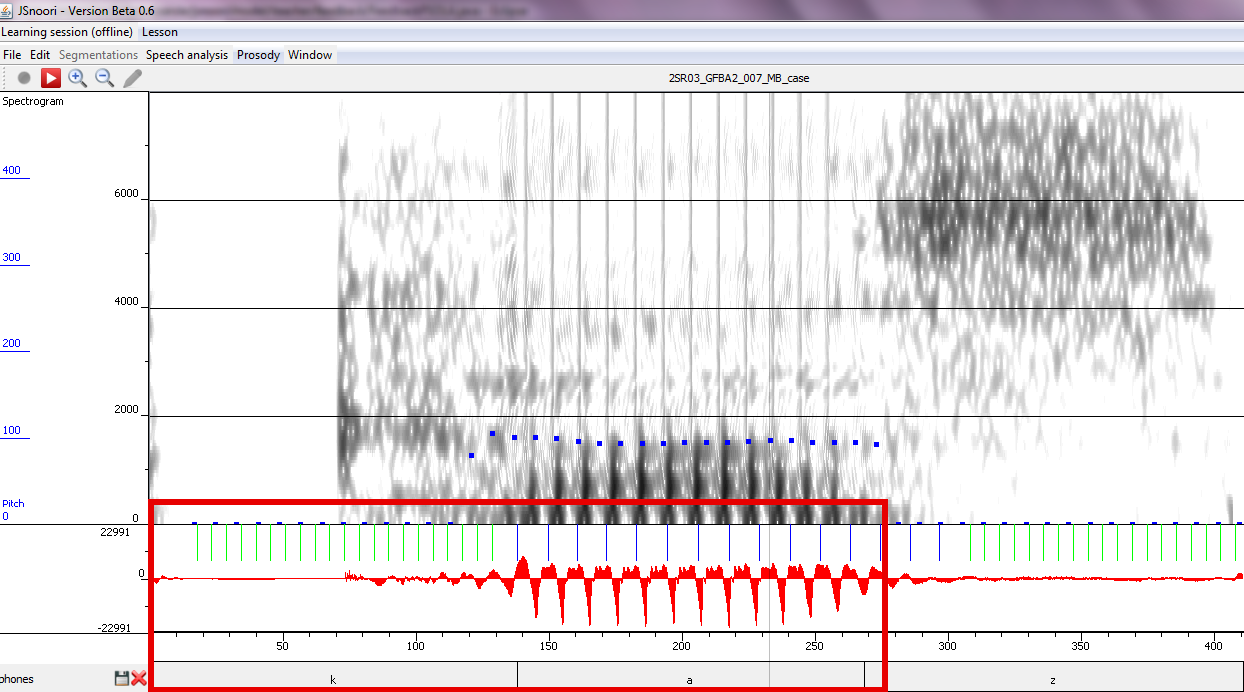
\includegraphics[width=0.9\linewidth]{images/case_learner-nonFricative.PNG}
  \caption{Pitch markers no-fricative extraction from the learner}
  \label{fig:sfig1}
\end{subfigure}%
\begin{subfigure}{.5\textwidth}
  \centering
  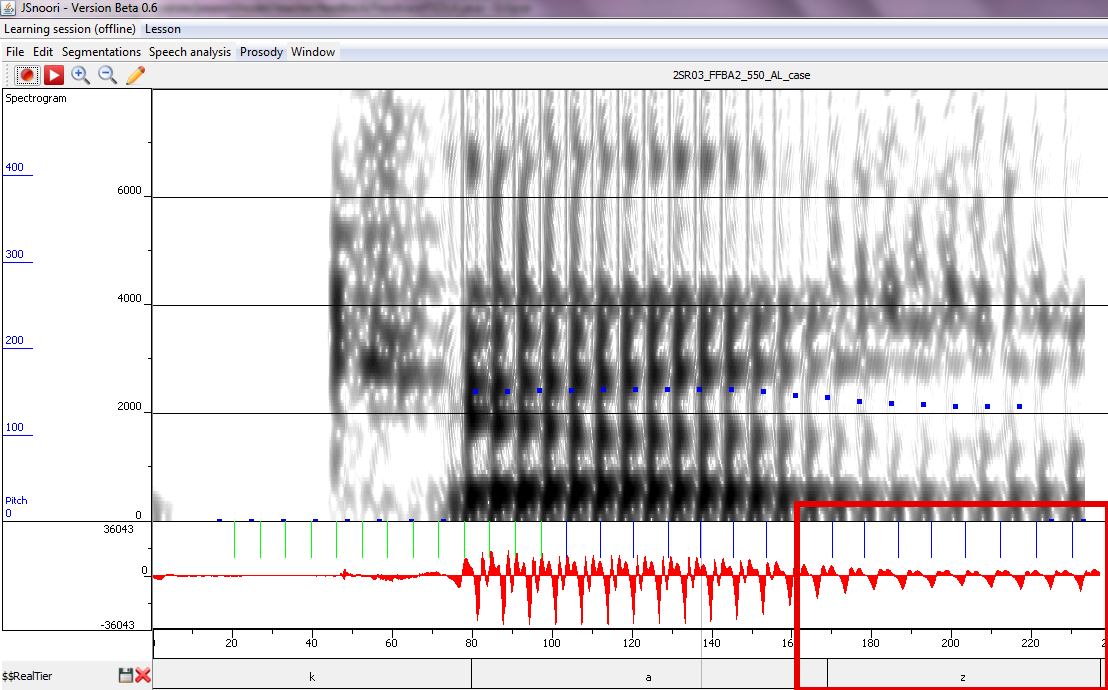
\includegraphics[width=0.9\linewidth]{images/teacher_case_pitchMarks.PNG}
  \caption{Pitch markers fricative extraction from the teacher}
  \label{fig:sfig2}
\end{subfigure}
\caption{Pitch Mark Extraction}
\label{fig:fig}
\end{figure}
\end{frame}

%%%%
\begin{frame}
\begin{figure}
%%%%%
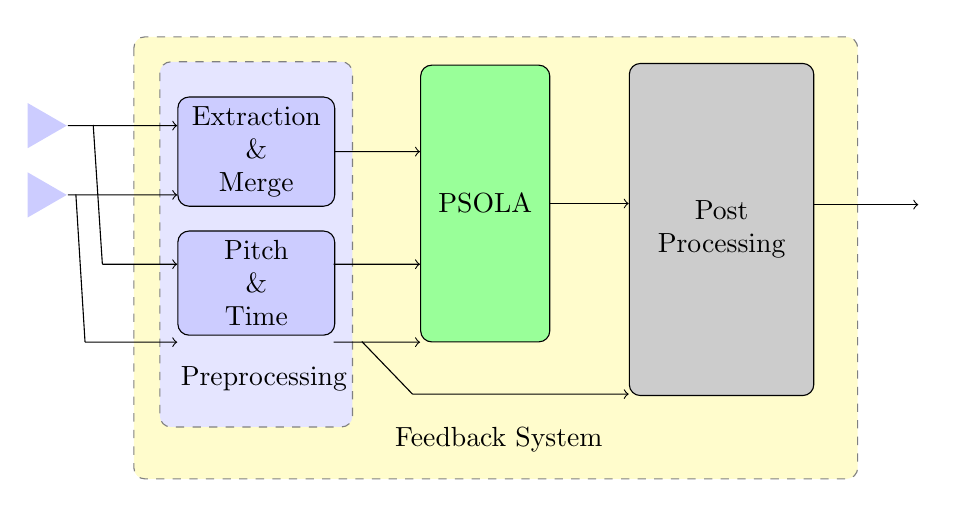
\begin{tikzpicture}[scale=1.1]
    \node (naveq) [naveqs={2}] {Post \\ Processing};
    % Note the use of \path instead of \node at ... below. 
     	
 	\path (naveq.0)+(-3.8,+0.3) node (psola) [psola={2}] {PSOLA};
      
    \path (naveq.140)+(-\blockdist,0) node (gyros) [block={2}] {Extraction \\ \& \\ Merge};
    \path (naveq.-150)+(-\blockdist,0) node (accel) [block={1}] {Pitch \\ \& \\ Time };
	\path (gyros.0)+(-3.4,+0.3) node (teacher) [input={1}] {};
    \path (gyros.0)+(-3.4,-0.5) node (learner) [input={1}] {};
 	
\path [draw, ->] (teacher) -- node [above] {} 
        (gyros.west |- teacher);
\path [draw, ->] (learner) -- node [above] {} 
        (gyros.west |- learner);
%\draw[<-] (accel.west) -- +(-0.8,0);
%\draw[<-] (accel.west) -- +(-0.8,0	);
\path (gyros.0)+(-2.8,-1.30) node (ref1){}; 
\path (gyros.0)+(-3.0,-2.2) node (ref2){};
%
\path (gyros.0)+(-2.8,+0.42) node (refTeacher){}; 
\path (gyros.0)+(-3.0,-0.38) node (refLearner){};
%
\path (gyros.east)+(-0.13,-1.30) node (pitch){}; 
\path (gyros.east)+(-0.13,-2.2) node (time){};
%
\path (gyros.east)+(+0.2,-2.080) node (ref1Pitch){}; 
\path (psola.west)+(-0.2,-2.2) node (ref2Pitch){}; 

%
%
%    \draw[->] (branch) node[branch] {}{}|- (ref1)




\path [draw, ->] (ref1) -- node [above] {} 
        (accel.west |- ref1);
 
\path [draw, ->] (ref2) -- node [above] {} 
        (accel.west |- ref2);

\path [draw, ->] (gyros) -- node [above] {} 
        (psola.west |- gyros);

\path [draw, -] (refTeacher)--(ref1.east);

\path [draw, -] (refLearner) -- (ref2.east);

\path [draw, ->] (pitch) -- node [above] {} 
        (psola.west |- pitch);

\path [draw, ->] (time) -- node [above] {} 
        (psola.west |- time);

\path [draw, ->] (ref2Pitch) -- node [above] {} 
        (naveq.west |- ref2Pitch);

\path [draw, -] (ref1Pitch) -- (ref2Pitch.east);

\path [draw, ->] (psola.east) -- node [above] {} 
        (naveq.west |- psola.east);
  
    % Unfortunately we cant use the convenient \path (fromnode) -- (tonode) 
    % syntax here. This is because TikZ draws the path from the node centers
    % and clip the path at the node boundaries. We want horizontal lines, but
    % the sensor and naveq blocks aren't aligned horizontally. Instead we use
    % the line intersection syntax |- to calculate the correct coordinate
   % \path [draw, ->] (gyros) -- node [above] {$\vc{\omega}_{ib}^b$} 
    %    (naveq.west |- gyros) ;
    % We could simply have written (gyros) .. (naveq.140). However, it's
    % best to avoid hard coding coordinates
    \path (accel.south west)+(+1.0,-0.5) node (IMU) {Preprocessing};
    \path (naveq.south west)+(-1.5,-0.5) node (INS) {Feedback System};
    \draw [->] (naveq.15	) -- node [ann={2}] {} + (\edgedist,0) 
        node[right] {};
%    \draw [->] (naveq.20) -- node [ann] {Attitude} + (\edgedist,0) 
   %     node[right] { $\mx{R}_l^b$};
%    \draw [->] (naveq.-25) -- node [ann] {Horisontal position} + (\edgedist,0)
   %     node [right] {$\mx{R}_e^l$};
%    \draw [->] (naveq.-50) -- node [ann] {Depth} + (\edgedist,0) 
%        node[right] {$z$};
    
    % Now it's time to draw the colored IMU and INS rectangles.
    % To draw them behind the blocks we use pgf layers. This way we  
    % can use the above block coordinates to place the backgrounds   
    \begin{pgfonlayer}{background}
        % Compute a few helper coordinates
        \path (gyros.west |- naveq.north)+(-0.5,0.3) node (a) {};
        \path (INS.south -| naveq.east)+(+0.5,-0.2) node (b) {};
        \path[fill=yellow!20,rounded corners, draw=black!50, dashed]
            (a) rectangle (b);
        \path (gyros.north west)+(-0.2,0.4) node (a) {};
        \path (IMU.south -| gyros.east)+(+0.2,-0.3) node (b) {};
        \path[fill=blue!10,rounded corners, draw=black!50, dashed]
            (a) rectangle (b);
    \end{pgfonlayer}
\end{tikzpicture}
\caption{Schema Block of Feedback Correction System }
\end{figure}
	\end{frame}





%%%%%%

\begin{frame}

\begin{figure}
\begin{subfigure}{.5\textwidth}
  \centering
  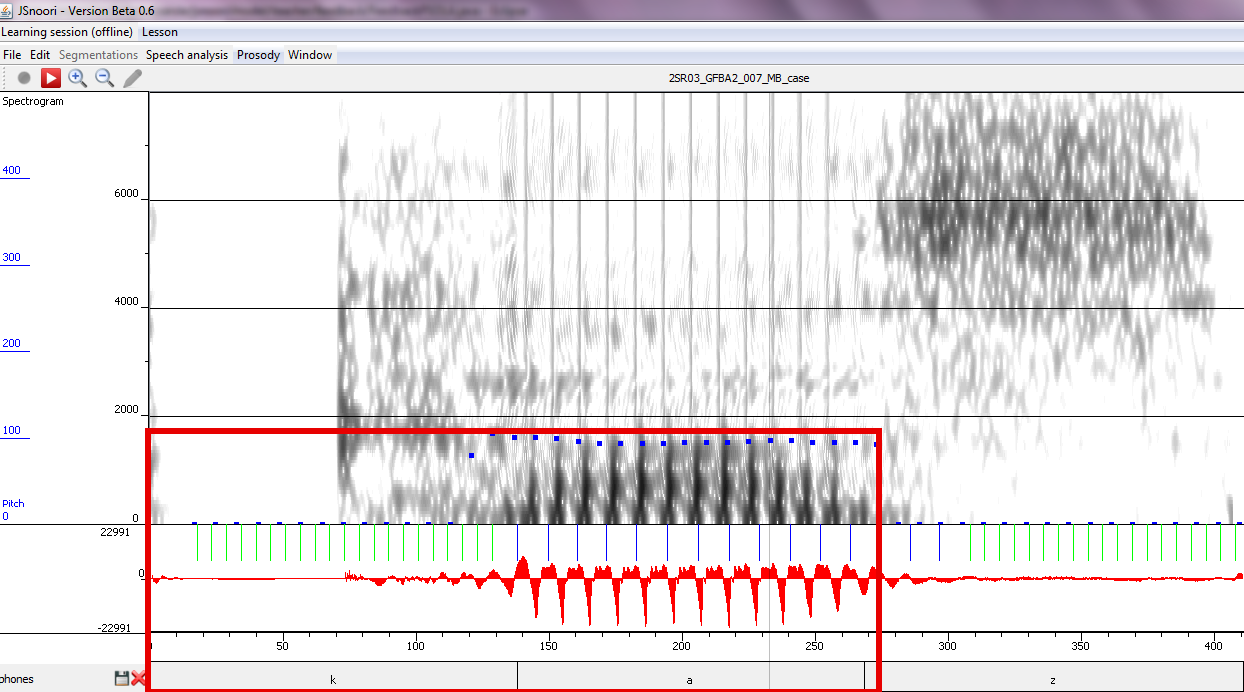
\includegraphics[width=0.9\linewidth]{images/case_learner-pitchMarkers.PNG}
  \caption{Learner signal before feedback correction}
  \label{fig:sfig1}
\end{subfigure}%
\begin{subfigure}{.5\textwidth}
  \centering
  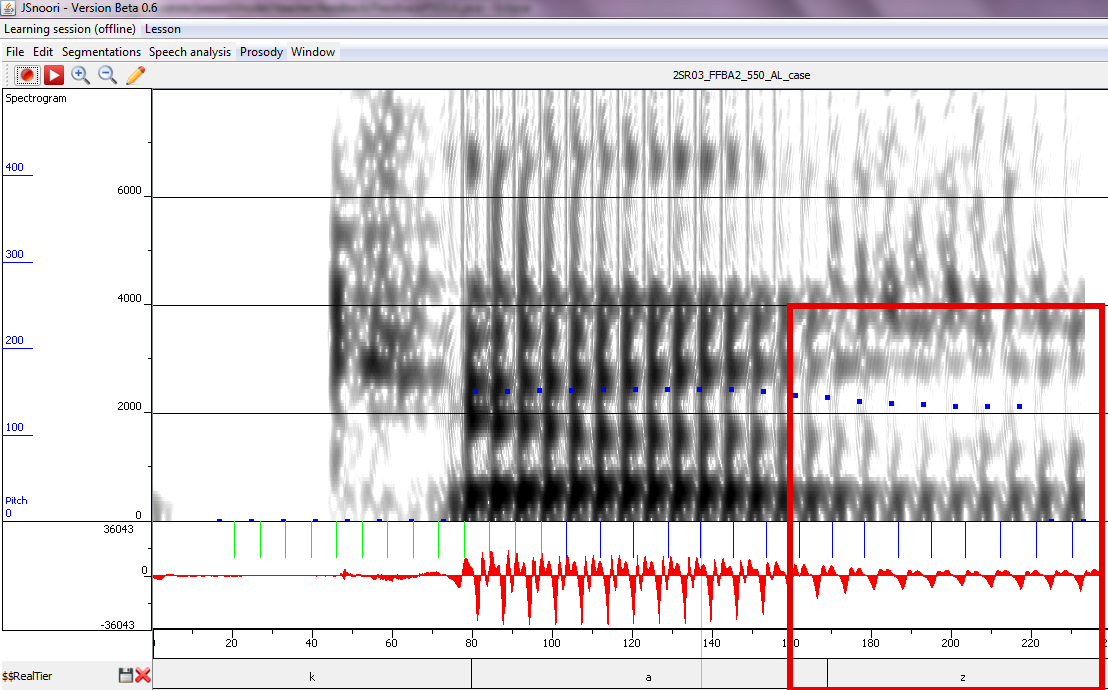
\includegraphics[width=0.9\linewidth]{images/teacher_case_Fricative.PNG}
  \caption{Teacher signal}
  \label{fig:sfig2}
\end{subfigure}
\caption{Pitch extraction and Time factor estimation}
\label{fig:fig}
\end{figure}
\end{frame}



%%%%%%%%

%% slide pitch & time 
\begin{frame}
\begin{figure}
%%%%%
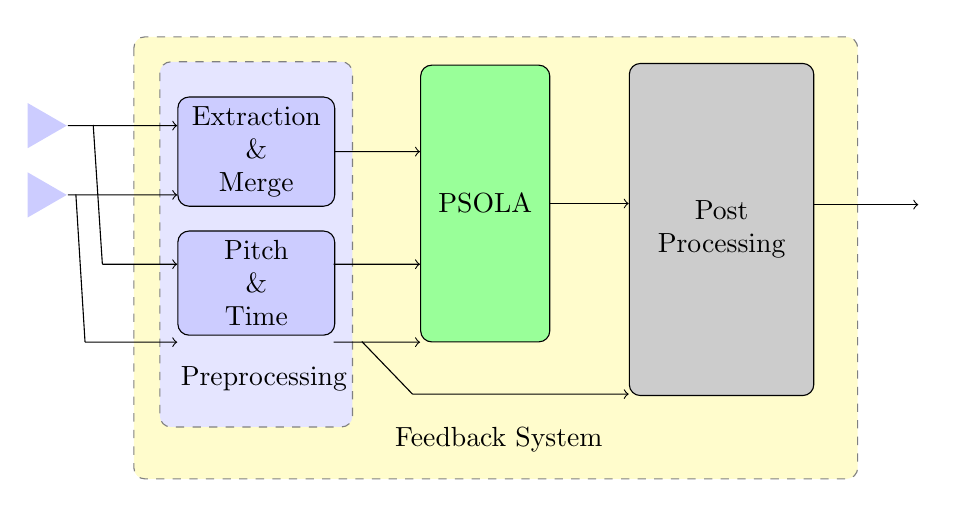
\begin{tikzpicture}[scale=1.1]
    \node (naveq) [naveqs={2}] {Post \\ Processing};
    % Note the use of \path instead of \node at ... below. 
     	
 	\path (naveq.0)+(-3.8,+0.3) node (psola) [psola={1}] {PSOLA};
      
    \path (naveq.140)+(-\blockdist,0) node (gyros) [block={2}] {Extraction \\ \& \\ Merge};
    \path (naveq.-150)+(-\blockdist,0) node (accel) [block={2}] {Pitch \\ \& \\ Time };
	\path (gyros.0)+(-3.4,+0.3) node (teacher) [input={1}] {};
    \path (gyros.0)+(-3.4,-0.5) node (learner) [input={1}] {};
 	
\path [draw, ->] (teacher) -- node [above] {} 
        (gyros.west |- teacher);
\path [draw, ->] (learner) -- node [above] {} 
        (gyros.west |- learner);
%\draw[<-] (accel.west) -- +(-0.8,0);
%\draw[<-] (accel.west) -- +(-0.8,0	);
\path (gyros.0)+(-2.8,-1.30) node (ref1){}; 
\path (gyros.0)+(-3.0,-2.2) node (ref2){};
%
\path (gyros.0)+(-2.8,+0.42) node (refTeacher){}; 
\path (gyros.0)+(-3.0,-0.38) node (refLearner){};
%
\path (gyros.east)+(-0.13,-1.30) node (pitch){}; 
\path (gyros.east)+(-0.13,-2.2) node (time){};
%
\path (gyros.east)+(+0.2,-2.080) node (ref1Pitch){}; 
\path (psola.west)+(-0.2,-2.2) node (ref2Pitch){}; 

%
%
%    \draw[->] (branch) node[branch] {}{}|- (ref1)




\path [draw, ->] (ref1) -- node [above] {} 
        (accel.west |- ref1);
 
\path [draw, ->] (ref2) -- node [above] {} 
        (accel.west |- ref2);

\path [draw, ->] (gyros) -- node [above] {} 
        (psola.west |- gyros);

\path [draw, -] (refTeacher)--(ref1.east);

\path [draw, -] (refLearner) -- (ref2.east);

\path [draw, ->] (pitch) -- node [above] {} 
        (psola.west |- pitch);

\path [draw, ->] (time) -- node [above] {} 
        (psola.west |- time);

\path [draw, ->] (ref2Pitch) -- node [above] {} 
        (naveq.west |- ref2Pitch);

\path [draw, -] (ref1Pitch) -- (ref2Pitch.east);

\path [draw, ->] (psola.east) -- node [above] {} 
        (naveq.west |- psola.east);
  
    % Unfortunately we cant use the convenient \path (fromnode) -- (tonode) 
    % syntax here. This is because TikZ draws the path from the node centers
    % and clip the path at the node boundaries. We want horizontal lines, but
    % the sensor and naveq blocks aren't aligned horizontally. Instead we use
    % the line intersection syntax |- to calculate the correct coordinate
   % \path [draw, ->] (gyros) -- node [above] {$\vc{\omega}_{ib}^b$} 
    %    (naveq.west |- gyros) ;
    % We could simply have written (gyros) .. (naveq.140). However, it's
    % best to avoid hard coding coordinates
    \path (accel.south west)+(+1.0,-0.5) node (IMU) {Preprocessing};
    \path (naveq.south west)+(-1.5,-0.5) node (INS) {Feedback System};
    \draw [->] (naveq.15	) -- node [ann={2}] {} + (\edgedist,0) 
        node[right] {};
%    \draw [->] (naveq.20) -- node [ann] {Attitude} + (\edgedist,0) 
   %     node[right] { $\mx{R}_l^b$};
%    \draw [->] (naveq.-25) -- node [ann] {Horisontal position} + (\edgedist,0)
   %     node [right] {$\mx{R}_e^l$};
%    \draw [->] (naveq.-50) -- node [ann] {Depth} + (\edgedist,0) 
%        node[right] {$z$};
    
    % Now it's time to draw the colored IMU and INS rectangles.
    % To draw them behind the blocks we use pgf layers. This way we  
    % can use the above block coordinates to place the backgrounds   
    \begin{pgfonlayer}{background}
        % Compute a few helper coordinates
        \path (gyros.west |- naveq.north)+(-0.5,0.3) node (a) {};
        \path (INS.south -| naveq.east)+(+0.5,-0.2) node (b) {};
        \path[fill=yellow!20,rounded corners, draw=black!50, dashed]
            (a) rectangle (b);
        \path (gyros.north west)+(-0.2,0.4) node (a) {};
        \path (IMU.south -| gyros.east)+(+0.2,-0.3) node (b) {};
        \path[fill=blue!10,rounded corners, draw=black!50, dashed]
            (a) rectangle (b);
    \end{pgfonlayer}
\end{tikzpicture}
\caption{Schema Block of Feedback Correction System }
\end{figure}
	\end{frame}


%%%%%%%%%%%%%%%%%
%% result befor post processing and after post processing
\begin{frame}
\frametitle{Post-processign}
\begin{figure}
\begin{subfigure}{.5\textwidth}
  \centering
  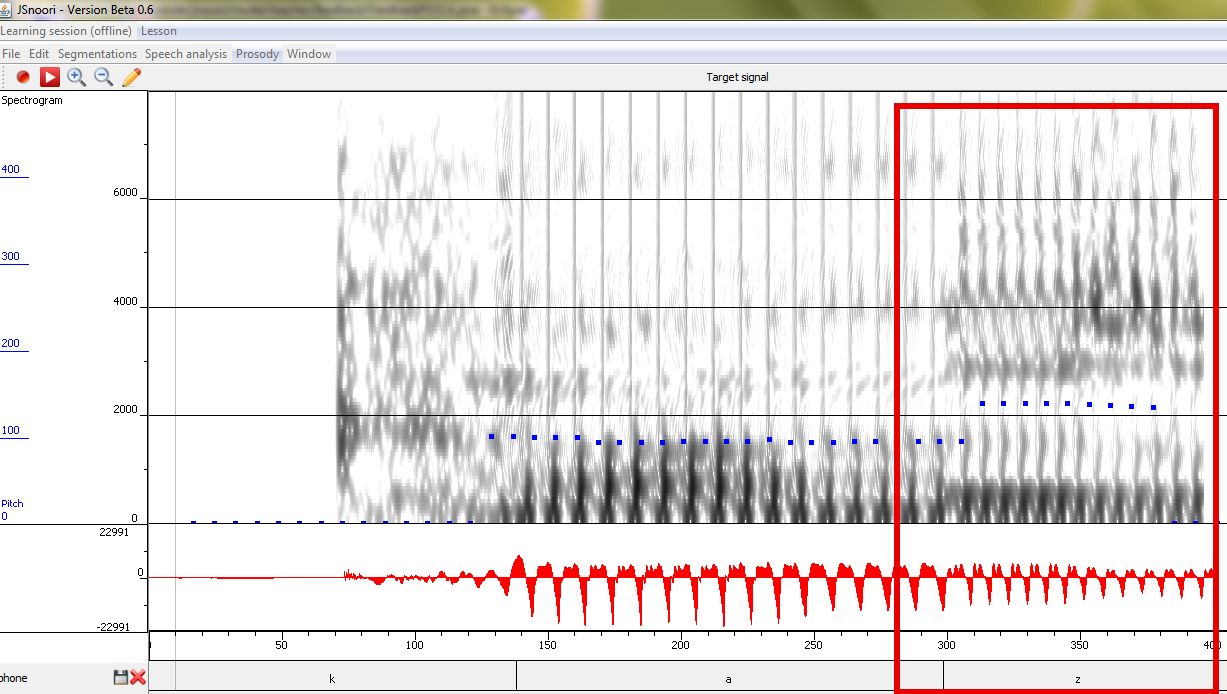
\includegraphics[width=0.9\linewidth]{images/target_befor_post_process1.PNG}
  \caption{Befor post-processing: pitch correction }
  \label{fig:sfig1}
\end{subfigure}%
\begin{subfigure}{.5\textwidth}
  \centering
  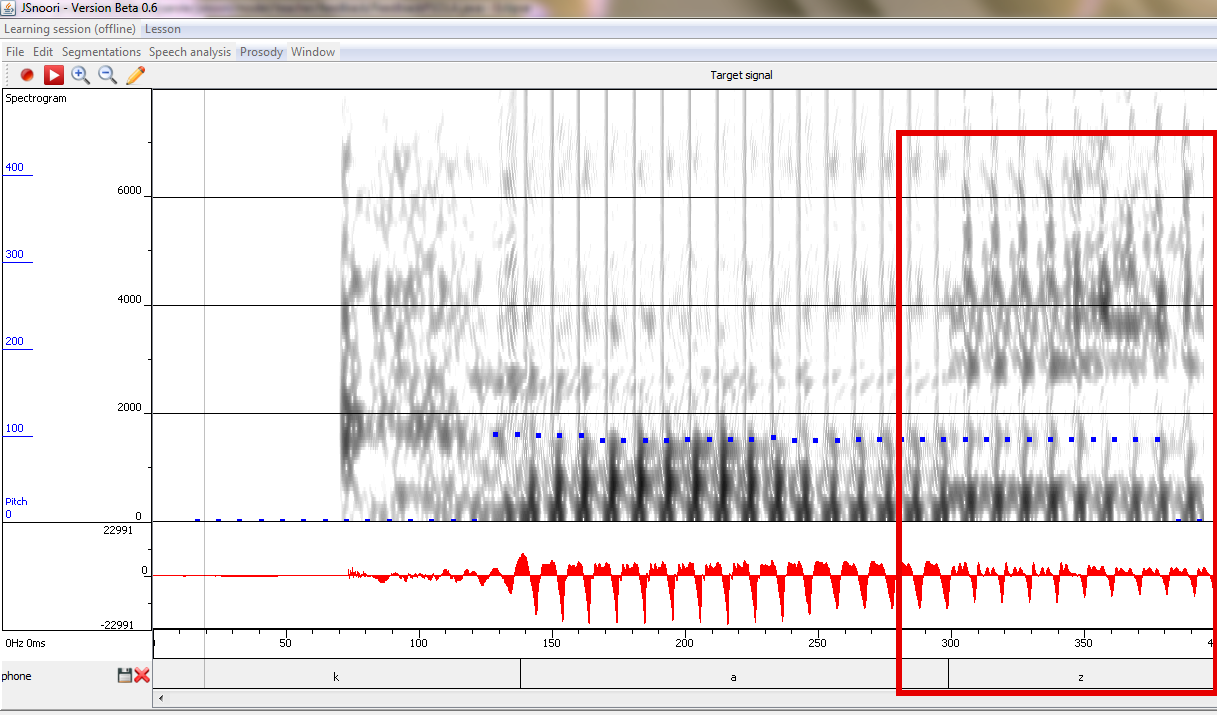
\includegraphics[width=0.9\linewidth]{images/case_target_2_changed.PNG}
  \caption{After Post-Processing}
  \label{fig:sfig2}
\end{subfigure}
\caption{Post-processing}
\label{fig:fig}
\end{figure}
\end{frame}



	
	
	
\end{document}